\documentclass[12pt]{article}
\usepackage{url}
\usepackage{tikz}
\usepackage{amsmath}
\usepackage{graphicx}
\usetikzlibrary{positioning}
\usepackage[margin=1in]{geometry}

\title{\vspace{-3em}Evolutionary Algorithms for Mechanical Structures}

\author{Tobias Jacob \\ Raffaele Galliera \\ Ali Muddasar}
\date{\today}

\begin{document}

\maketitle

\begin{abstract}
\centering
We want to develop a program that improves mechanical structures using an evolutionary algorithm.
\end{abstract}

We have always wondered how to simulate continues mechanics and how to use evolutionary algorithms to solve engineering problems. An evolutionary algorithm is supposed to generate a 2D mechanical structure and then evaluate if it can withstand a certain force.

\begin{figure}[h]
    \centering
    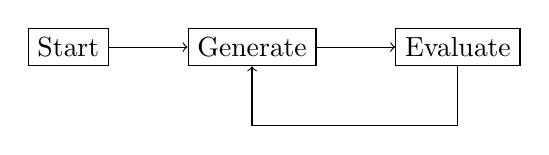
\begin{tikzpicture}
        \node[draw] (start) {Start};
        \node[right=of start, draw] (generate) {Generate};
        \node[right=of generate, draw] (evaluate) {Evaluate};

        \draw[->] (start) -- (generate);
        \draw[->] (generate) -- (evaluate);
        \draw[->] (evaluate) -- +(0, -1cm) -| (generate);
    \end{tikzpicture}
\end{figure}

Each mechanical structure is represented by a 2D Boolean array, like the following.

\begin{figure}[h]
    \centering
    \begin{tabular}{cccc}
        0 & 0 & 0 & 0 \\
        0 & 0 & 1 & 0 \\
        1 & 1 & 1 & 1 \\
        0 & 0 & 0 & 0
    \end{tabular}
\end{figure}

A $1$ is indicating that there is a quadratic element (consisting out of two triangles). We may fine tune the generation of triangles from the grid. The structures get evaluated on withstanding a certain force using finite elements method. We just use rectangular isosceles triangles with side length 1, simplifying the equations. Figure \ref{fig:finiteElements} shows the results of a test python implementation we created. It is based on the explanations in~\cite[p. 15-22]{Nikishkov2004}.

Different models will be evaluated if they can withstand a certain force by simulation. Then, according to the evolutionary approach we are taking, the best ones get paired and produce children that are similar, but have random mutations and alterations.

Each model can be simulated on a different node. The simulation itself requires solving a linear equation system with a big sparse, symmetric and positive definite matrix. For a $R \times C$ grid, it would contain ${2RC}$ rows. Solving the equation can be parallelized across multiple cores of each node. After each model has been simulated, all workers must submit their test-scores. Then, new models have to be generated and the simulation runs again.


\bibliographystyle{abbrv}
\bibliography{description}

\begin{figure}[p]
    \centering
    \includegraphics[width=0.5\textwidth, trim={0cm 6.5cm 0cm 0cm}, clip]{images/finiteElements.pdf}
    \caption{Example of a finite element simulation. Green is the original shape, Red is the deformed structure after reacting to the blue force.}
    \label{fig:finiteElements}
\end{figure}

\begin{figure}[p]
    \centering
    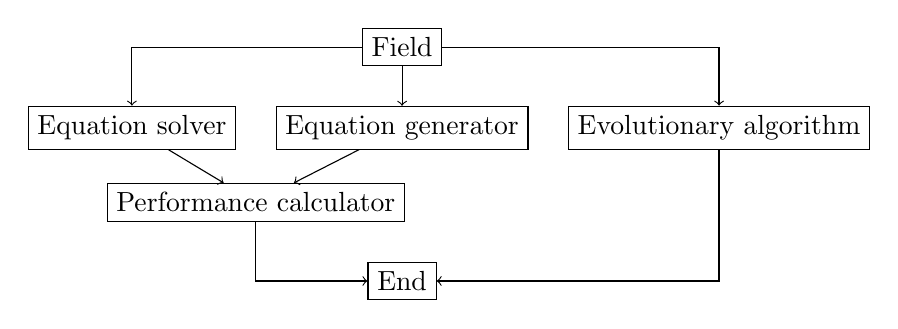
\begin{tikzpicture}
        \node[draw] (start) {Field};
        \node[below=0.5cm of start, draw] (generator) {Equation generator};
        \node[left=0.5cm of generator, draw] (solve) {Equation solver};
        \path (solve) -- node [below=0.7cm, draw] (performance) {Performance calculator} (generator);
        \node [right = 0.5cm of generator, draw] (evolution) {Evolutionary algorithm};
        \node [below of=0.5cm, draw] at (start|-performance) (end) {End};
        \draw[->] (start) -| (solve);
        \draw[->] (start) -- (generator);
        \draw[->] (start) -| (evolution);
        \draw[->] (solve) -- (performance);
        \draw[->] (generator) -- (performance);
        \draw[->] (performance) |- (end);
        \draw[->] (evolution) |- (end);
    \end{tikzpicture}
    \caption{Our planned workflow.}
    \label{fig:workflow}
\end{figure}

\end{document}